% if there are questions please contact me:
% lars.bilke@ufz.de

\newcommand{\ogs}{OpenGeoSys }

\chapter{Software engineering}
\textit{by Lars Bilke}

\bigskip

The \ogs software development community is distributed all over the world and people with different backgrounds contribute code to a complex software system. The following points have to be addressed for a successful software development:

\begin{itemize}\addtolength{\itemsep}{-0.3\baselineskip}
\item Platform independent code
\item A single build system
\item A version control system
\item A collaborative project web site
\item Continuous builds and testing
\item Providing binaries and documentation for end users
\end{itemize}

\ogs should run on a PC as well as on a computing cluster regardless of the operating system. Therefore the code should not include any platform specific feature or library. Instead open source and platform independent libraries like Qt\footnote{Qt: \texttt{http://qt.nokia.com/products/}} for the graphical user interface or VTK\footnote{The Visualization Toolkit: \texttt{http://www.vtk.org}} for visualization algorithms are used. So developers can simply use the platform or tools they want.

Despite the use of platform independent code and libraries, in the end there must be platform specific build settings or project files for integrated development environments like Visual Studio or Eclipse. These are generated by the CMake\footnote{CMake: \texttt{http://www.cmake.org}} build system which is configured using platform independent configuration files. Also, CMake enables so-called \emph{out of source builds} which means that all the generated files are separated from the source code. This makes it easier to manage the source code in a version control system.

A source code management and version control system is a definite requirement for distributed software development. For this purpose Subversion\footnote{Subversion: \texttt{http://subversion.tigris.org/}} is used which enables developers to work on separate versions (\emph{branches}) of the software and to merge those versions at some point to the official one.

The version control system is integrated into an information and collaboration website based on a wiki\footnote{TracWiki: \texttt{http://trac.edgewall.org/wiki/TracWiki}} system. The wiki is used for collecting informations such as tutorials, application examples and case studies. Discussions take place in the \ogs mailing list\footnote{OGS-Mailinglist: \texttt{http://groups.google.com/group/ogs6}}.

To improve code stability and to verify code correctness a continuous build and testing system based on the Jenkins Continuous Integration Server\footnote{Jenkins: \texttt{http://jenkins-ci.org/}} has been established. This server is connected to the version control system and does the following on every code change:

\begin{itemize}\addtolength{\itemsep}{-0.3\baselineskip}
\item Compiles (\emph{builds}) the code on every supported platform (Linux, Windows, MacOS)
\item Runs a comprehensive test suite of over 120 benchmarks
\item Verifies the test results
\item Runs software development related metrics on the code (like compiler warnings, code complexity, static analysis tools)
\item Generates source code documentation
\item Provides binaries for end users
\item Informs developers on errors
\end{itemize}

These points enhance the software development process considerably. The platform independence is maintained. Errors in the source code can be tracked down easily and at the time they were introduced. Developers get access to code analysis tools and an up-to-date source code documentation without the need to install it on their own machines.

Figure \ref{fig:lb:engineering-workflow} shows an overview of the software engineering workflow and concludes this section.

\begin{figure}[tb]
\begin{center}
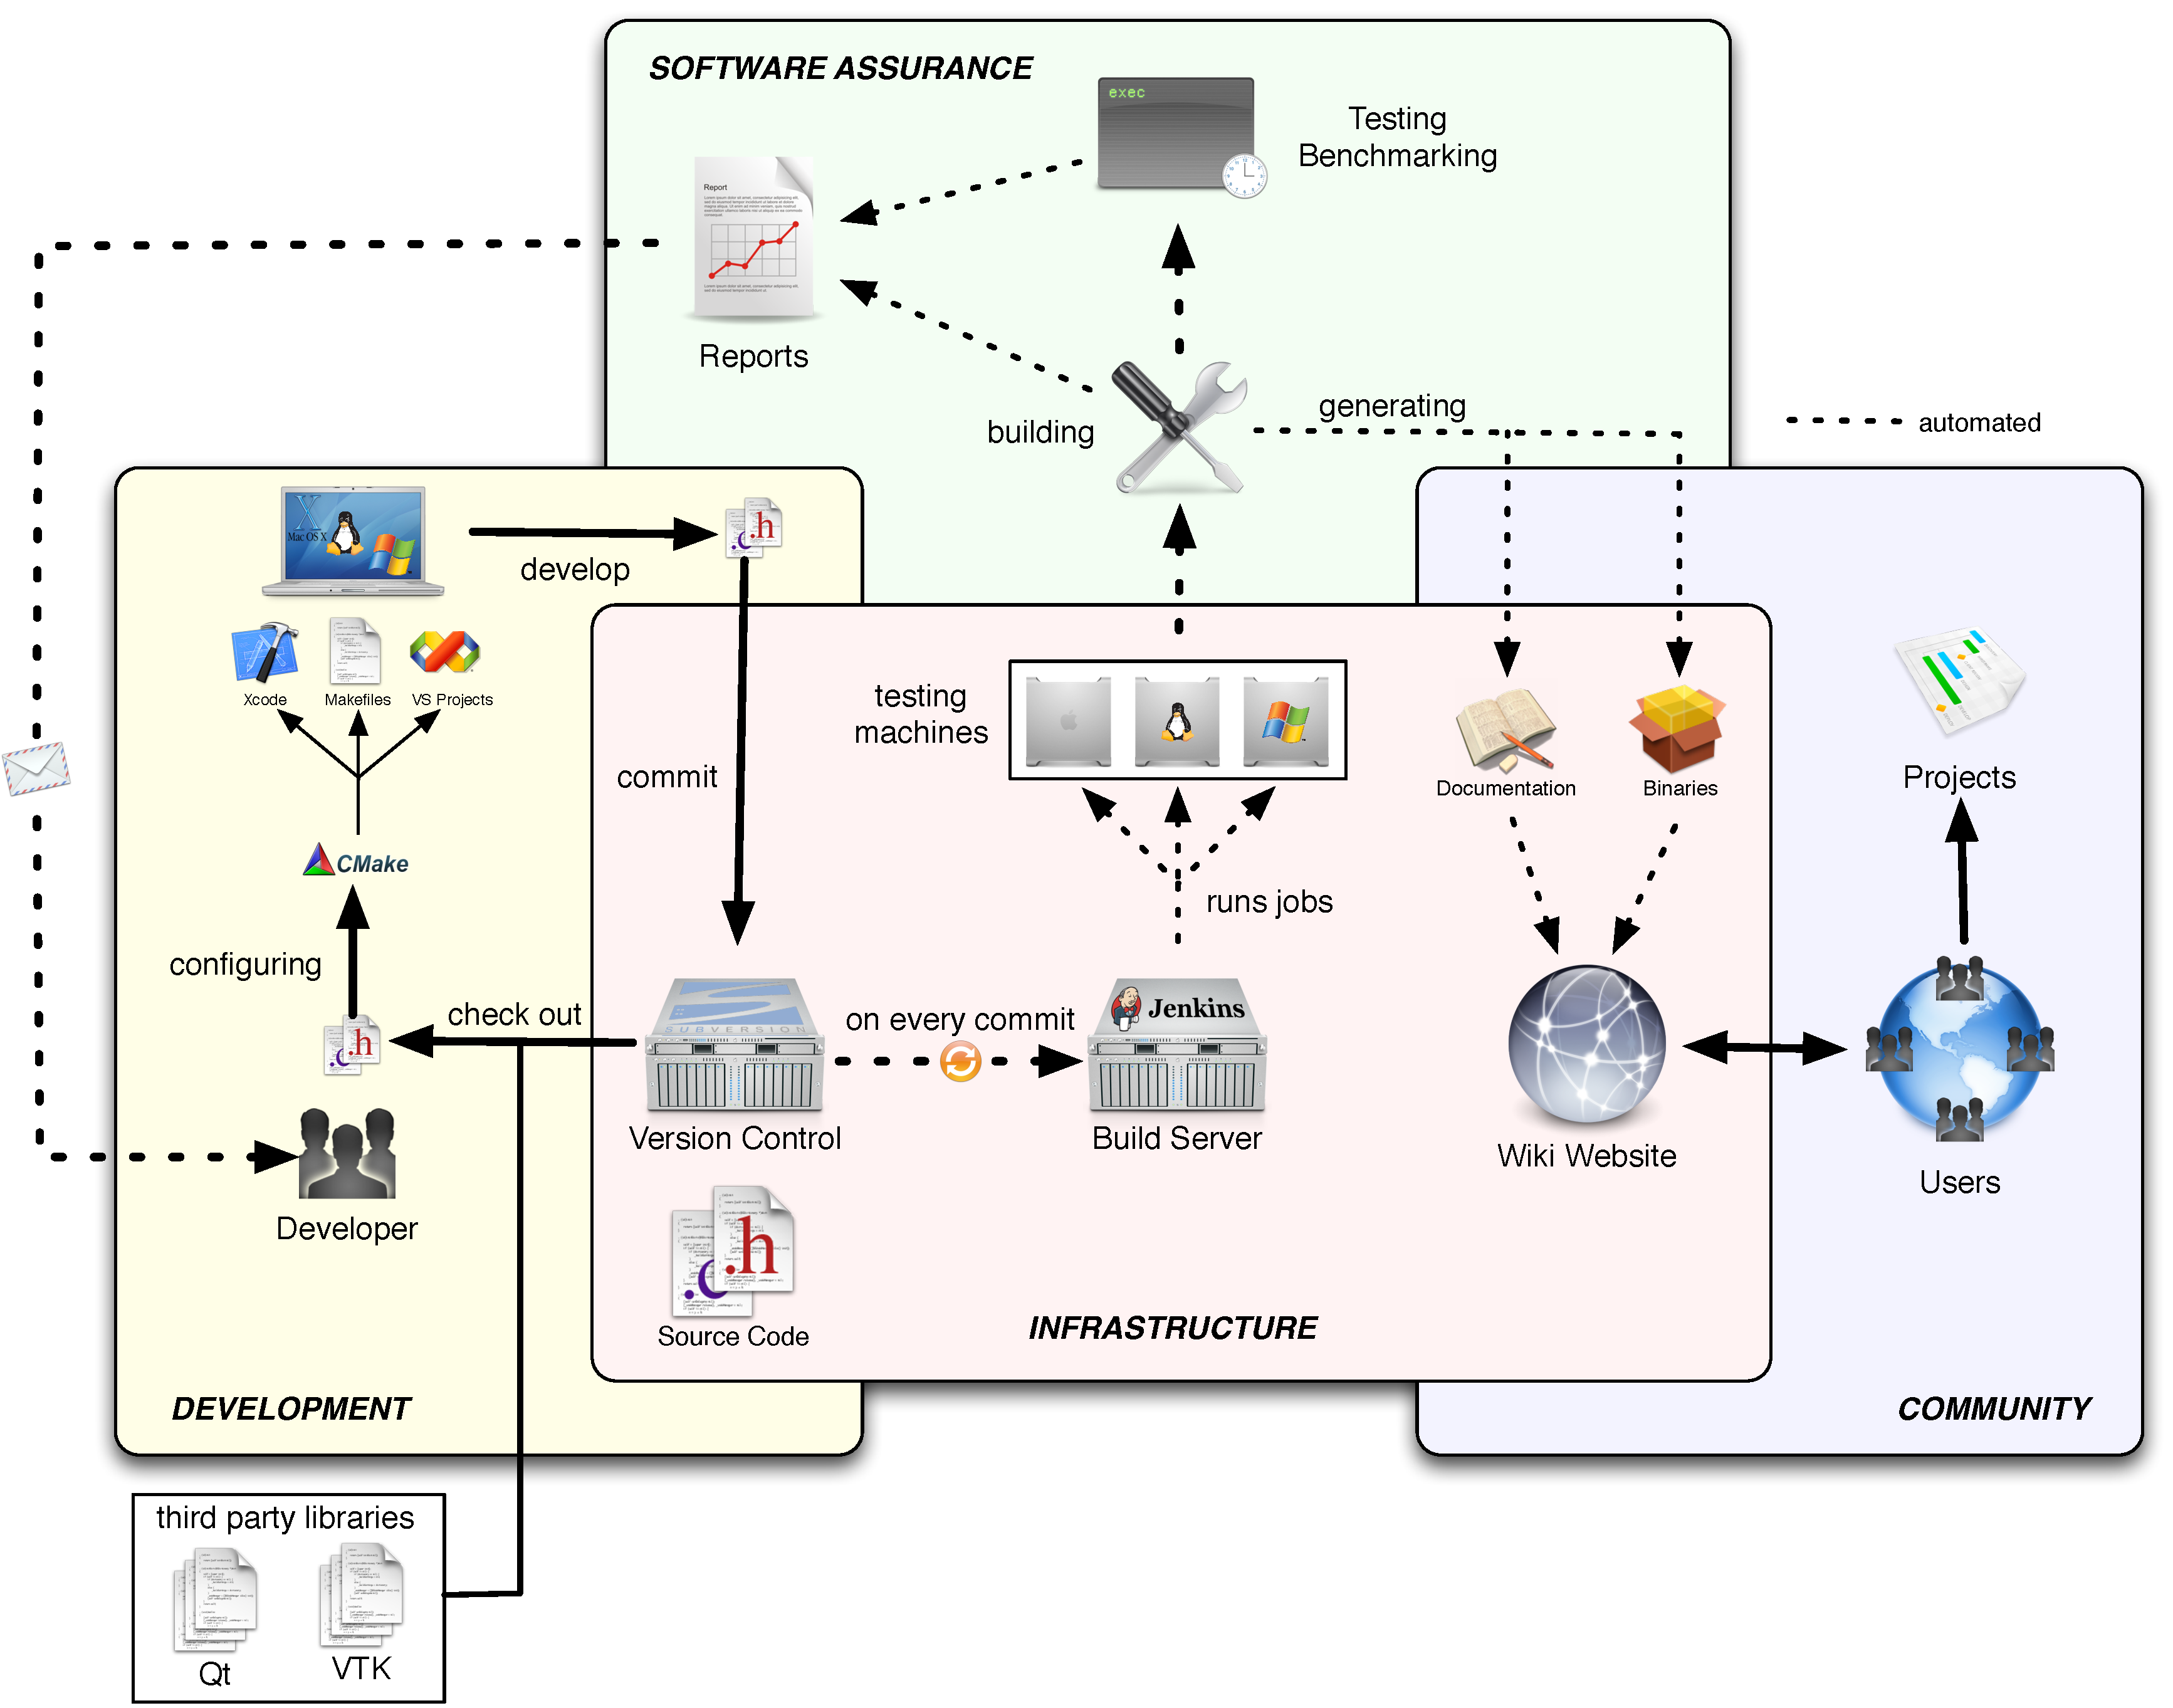
\includegraphics[width=0.99\linewidth]{figures/engineering-workflow}
\caption{Overview of the \ogs software engineering workflow.}
\label{fig:lb:engineering-workflow}
\end{center}
\end{figure}
